\chapter{Capitolul 8}
\section{PromON}
%%poza siglaaa!!!
\textbf{Log In/Sign Up}
\paragraph{ }Meniul de start al aplicației client este reprezentat de fereastra de Log In/Sign Up care este afișată doar în cazul în care utilizatorul nu este deja autentificat. Aceasta cuprinde două text box-uri în care clientul își va introduce un e-mail și o parolă necesare pentru autentificare sau pentru crearea unui cont nou, caz în care va fi necesară o confirmare a parolei.

\begin{center}
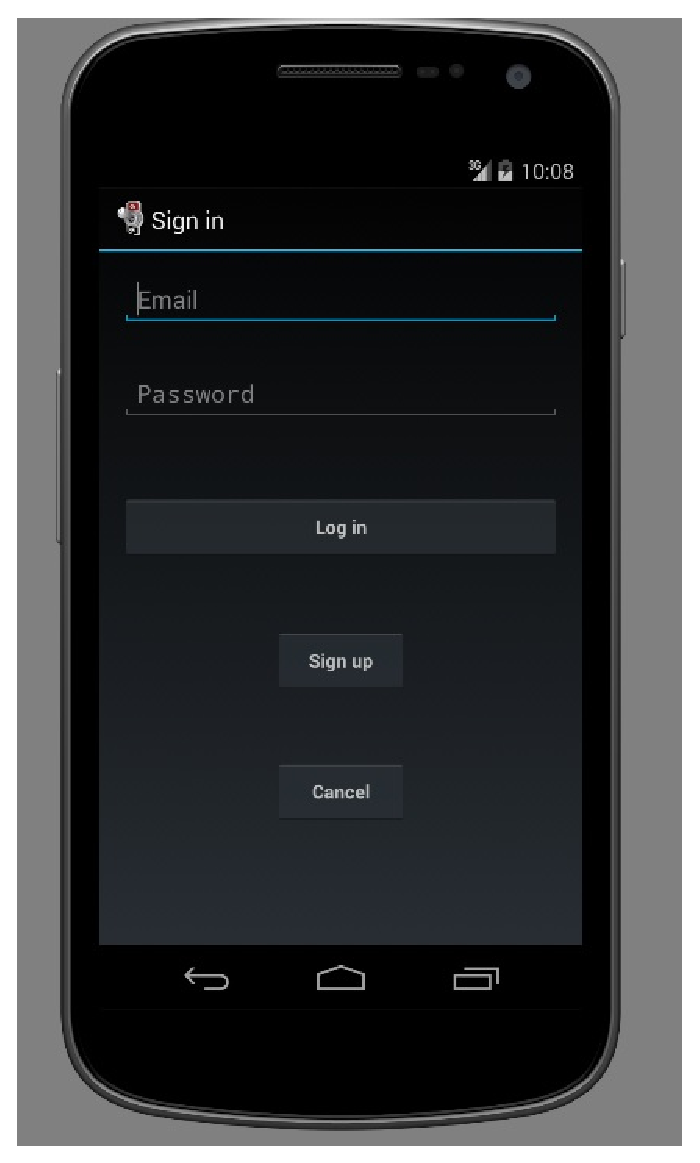
\includegraphics[width=12cm,height=9cm,keepaspectratio]{imagini/login.eps} %&
\paragraph{}
\textbf{Login}
\end{center}

\begin{center}
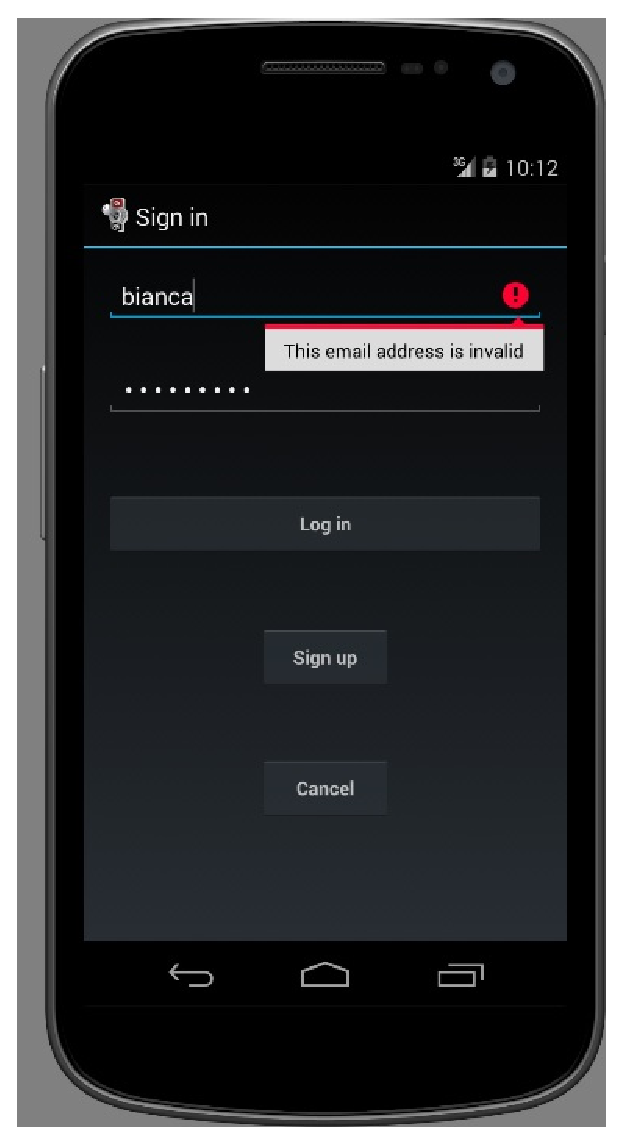
\includegraphics[width=12cm,height=9cm,keepaspectratio]{imagini/emailinvalid.eps} %&
\paragraph{}
\textbf{Atenționare e-mail invalid}
\end{center}

\begin{center}
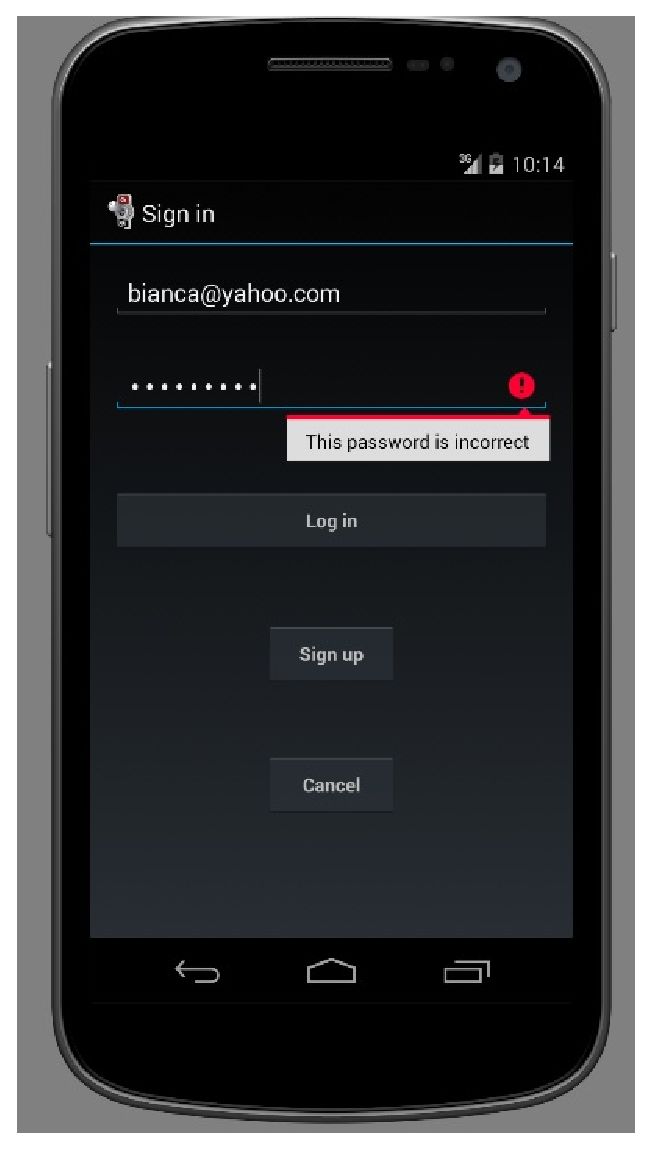
\includegraphics[width=12cm,height=9cm,keepaspectratio]{imagini/invalidpass.eps} %&
\paragraph{}
\textbf{Atenționare parolă invalidă}
\end{center}

\textbf{Pagina principală}
\paragraph{ }După conectare se va deschide o pagină în care, vor fi afișate primele 10 produse sortate în funcție de cel mai mare discount acordat. Acestea se vor schimba dupa 5 secunde timp în care dacă utilizatorul este interesat va putea apăsa pe butonul ,,cumpără'' care îl va redirecționa spre site-ul de unde poate achiziționa produsul.

\textbf{Meniul slide-in}
\paragraph{ }Pentru a oferi un design elegant și nu foarte încărcat, pentru a naviga prin celelalte funcționalități ale aplicației am ales să utilizez un meniu slider care va sta ascuns pe parcursul acțiunilor de pe o anumită pagină dar va putea fi oricând vizibil printr-o simplă atingere a ecranului dinspre stânga spre dreapta sau prin atingerea iconiței de meniu. Astfel toate modulele aplicației sunt grupate și pot fi accesate rapid și simplu, comunicarea între acestea fiind de asemenea printr-o simpla atingere a elementului din meniu corespunzător paginii care se dorește a fi deschisă.
Unul dintre motivele pentru care am ales să dezvolt aplicația pentru versiunile de Android pornind de la IceCreamSandwich este utilizarea acestui tip de meniu care din punctul meu de vedere are un impact mare fiind un instrument modern și din ce în ce mai utilizat în aplicații importante precum Facebook, YahooMail, GMail etc. Asfel, utilizatorii Android sunt obișnuiți cu utilizarea acestui navigator și pot folosi aplicația cu ușurință. 
%poza meniul meu si eventual poza meniu fb, mail?

\textbf{Categorii}
 \paragraph{ }Acest fragment al aplicației cuprinde o listă de categorii de produse disponibile, personalizate cu o iconiță sugestivă pentru impact vizual și un buton comutator prin care un client își poate alege metoda de afișare a categoriilor, sortate în funcție de nume, alfabetic, sau în functie de numărul de accesări, cele mai populare categorii fiind listate primele în acest caz.
\begin{center}
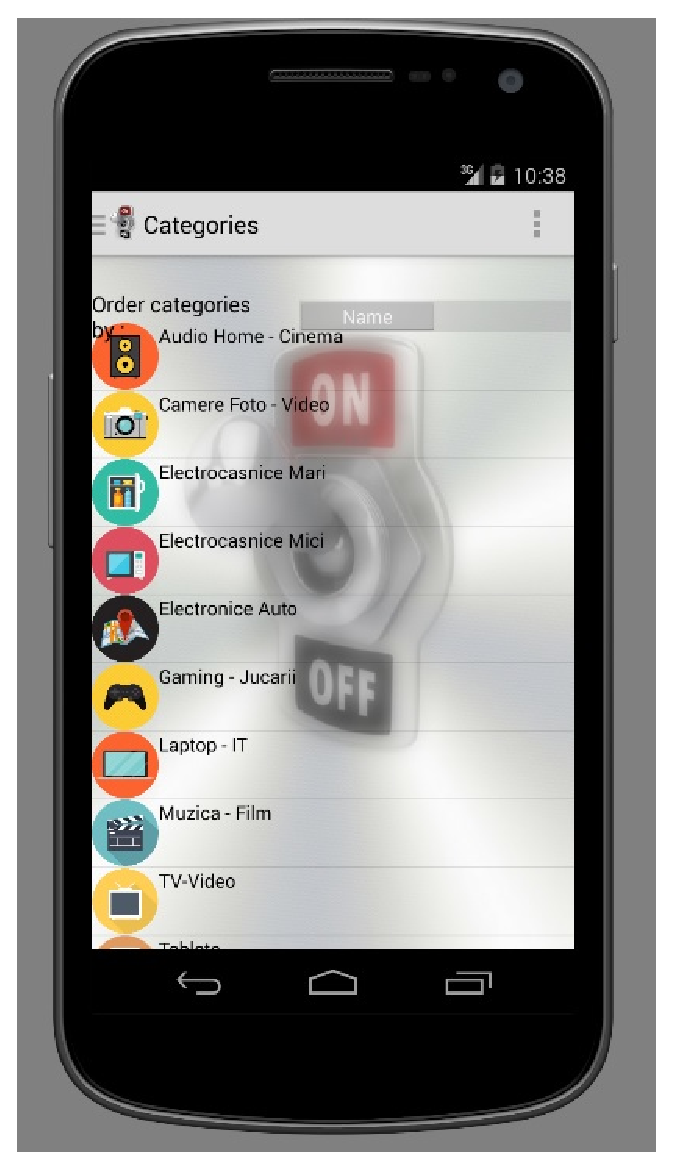
\includegraphics[width=12cm,height=9cm,keepaspectratio]{imagini/categorii.eps} %&
\paragraph{}
\textbf{Listă categorii sortate alfabetic}
\end{center}

\begin{center}
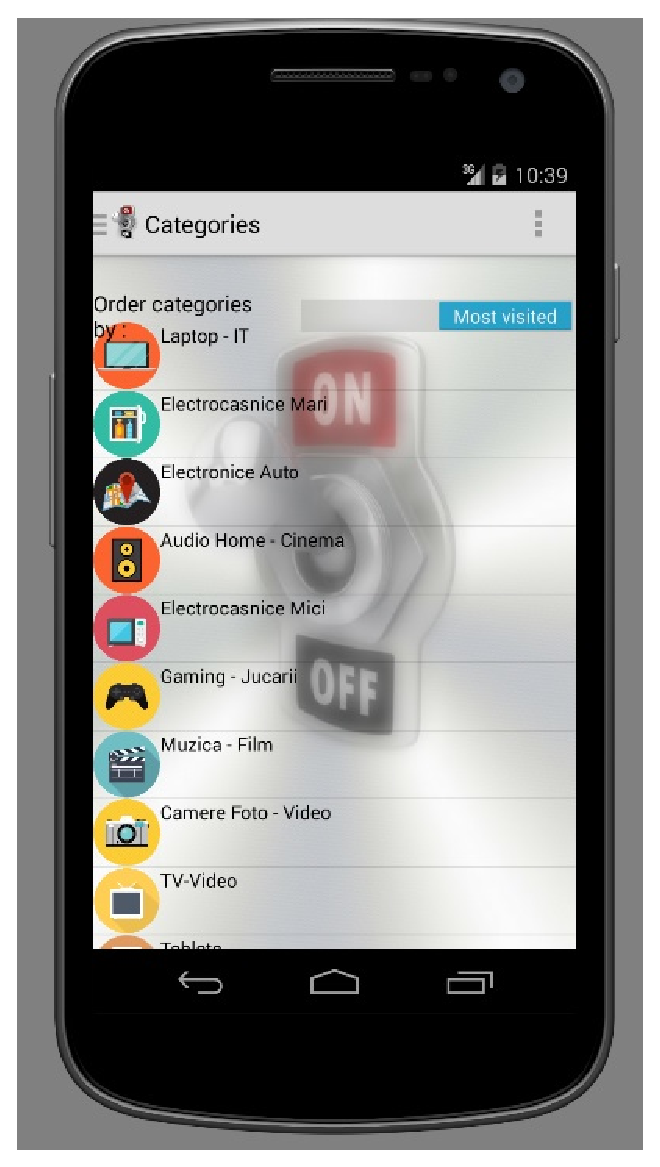
\includegraphics[width=12cm,height=9cm,keepaspectratio]{imagini/catgorii2.eps} %&
\paragraph{}
\textbf{Listă categorii sortate în funcție de numărul de accesări}
\end{center}

\textbf{Produse}
\paragraph{ }După ce utilizatorul selectează o categorie din listă, se deschide o nouă fereastră, ce cuprinde o listă cu produsele care apartin categoriei alese. De asemenea acestea pot fi sortate, utilizând un buton comutator, alfabetic sau descrescător după valoarea discountului care se oferă pentru fiecare produs în parte.
După ce alege produsul dorit, pentru a fi vizionat în detaliu se deschide o nouă fereastră în care se pot vizualiza prețul curent, prețul anterior, detalii despre produs și o poză semnificativă.  Această pagină corespunde cu pagina principală, în care sunt afișate însă doar 10 produse, considerate produsele de top. De asemenea, pentru a cumpăra un produs, apare un buton, care , o dată apăsat va deschide browserul principal al telefonului și va deschide pagina corespunzătoare produsului curent.

\textbf{Setări}
\paragraph{ } Meniul de setări cuprinde opțiunea de a alege o temă pentru aplicație prin selectarea acesteia dintr-un meniu drop-down. O dată selectată o temă, clientul trebuie să apese butonul Aplică pentru ca tema curentă să se modifice cu cea aleasă.  Acest fragment de aplicație este oferă posibilitatea utilizatorul de a-si personaliza aplicația, este util însă și pentru sănătatea ochilor întrucât în funcție de lumină este recomandat să alegem culori care să nu ne afecteze vederea. 

\begin{center}
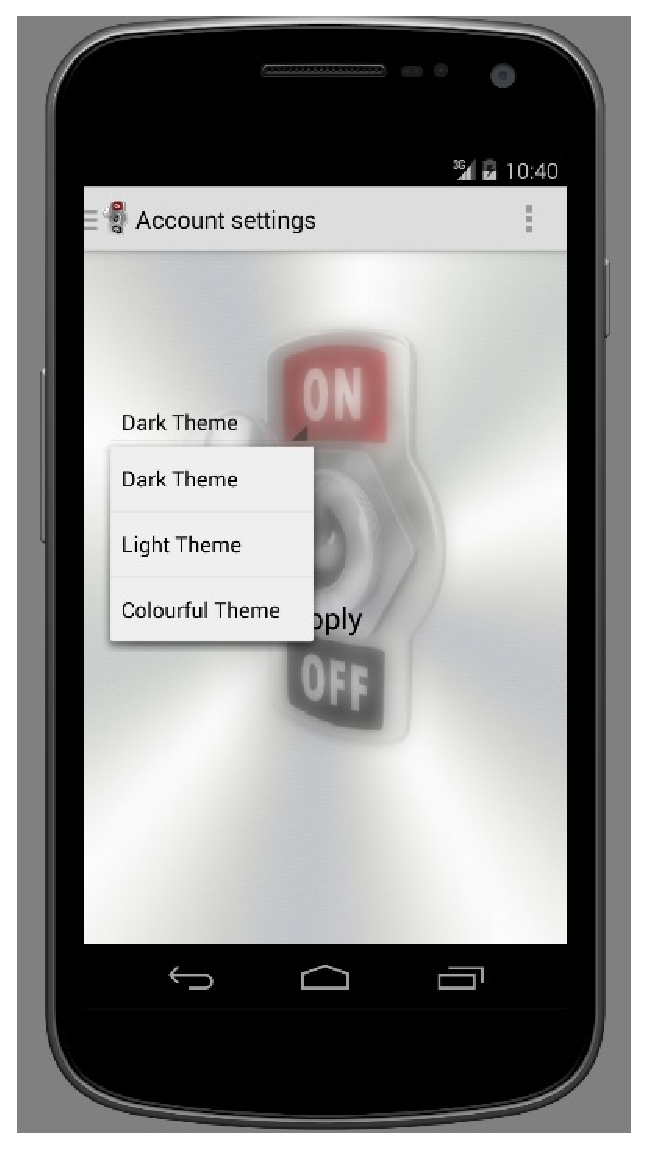
\includegraphics[width=12cm,height=9cm,keepaspectratio]{imagini/settings.eps} %&
\paragraph{}
\textbf{Pagină setări}
\end{center}

\textbf{Termeni și condiții}
\paragraph{ } Orice aplicație cuprinde o serie de termeni și condiții, aceștia au fost acceptați o dată cu instalarea aplicației, însă este de preferat să fie disponibili pentru o recitire ulterioară și în cazul în care utilizatorul nu este de acord să poată dezinstala aplicația.


\textbf{Log Out}
\paragraph{ } Acest fragment se referă la ieșirea din cont și o dată apăsat butonul de Log Out, utilizatorul va fi redirecționat către pagina de Log In, unde va putea să se autentifice cu un alt cont deja existent, să-și creeze un cont nou sau pur și simplu să iasă din aplicație.
\begin{center}
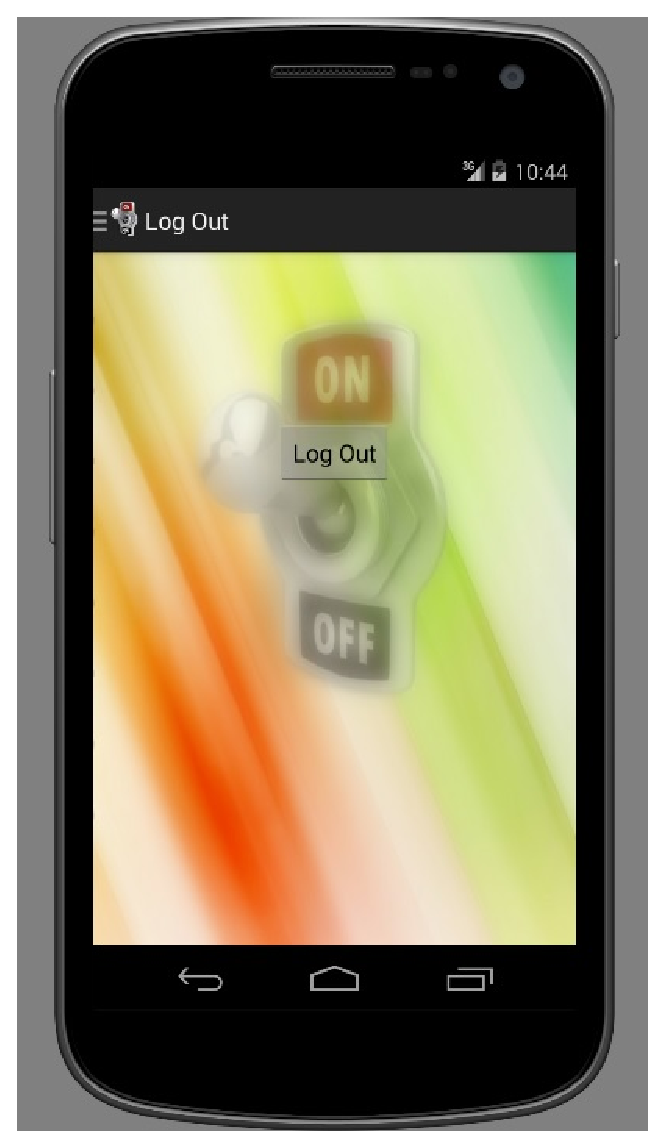
\includegraphics[width=12cm,height=9cm,keepaspectratio]{imagini/logout.eps} %&
\paragraph{}
\textbf{Pagină log out}
\end{center}


%%%%Find a product????

